% Options for packages loaded elsewhere
% Options for packages loaded elsewhere
\PassOptionsToPackage{unicode}{hyperref}
\PassOptionsToPackage{hyphens}{url}
\PassOptionsToPackage{dvipsnames,svgnames,x11names}{xcolor}
%
\documentclass[
]{article}
\usepackage{xcolor}
\usepackage{amsmath,amssymb}
\setcounter{secnumdepth}{-\maxdimen} % remove section numbering
\usepackage{iftex}
\ifPDFTeX
  \usepackage[T1]{fontenc}
  \usepackage[utf8]{inputenc}
  \usepackage{textcomp} % provide euro and other symbols
\else % if luatex or xetex
  \usepackage{unicode-math} % this also loads fontspec
  \defaultfontfeatures{Scale=MatchLowercase}
  \defaultfontfeatures[\rmfamily]{Ligatures=TeX,Scale=1}
\fi
\usepackage{lmodern}
\ifPDFTeX\else
  % xetex/luatex font selection
\fi
% Use upquote if available, for straight quotes in verbatim environments
\IfFileExists{upquote.sty}{\usepackage{upquote}}{}
\IfFileExists{microtype.sty}{% use microtype if available
  \usepackage[]{microtype}
  \UseMicrotypeSet[protrusion]{basicmath} % disable protrusion for tt fonts
}{}
\makeatletter
\@ifundefined{KOMAClassName}{% if non-KOMA class
  \IfFileExists{parskip.sty}{%
    \usepackage{parskip}
  }{% else
    \setlength{\parindent}{0pt}
    \setlength{\parskip}{6pt plus 2pt minus 1pt}}
}{% if KOMA class
  \KOMAoptions{parskip=half}}
\makeatother
% Make \paragraph and \subparagraph free-standing
\makeatletter
\ifx\paragraph\undefined\else
  \let\oldparagraph\paragraph
  \renewcommand{\paragraph}{
    \@ifstar
      \xxxParagraphStar
      \xxxParagraphNoStar
  }
  \newcommand{\xxxParagraphStar}[1]{\oldparagraph*{#1}\mbox{}}
  \newcommand{\xxxParagraphNoStar}[1]{\oldparagraph{#1}\mbox{}}
\fi
\ifx\subparagraph\undefined\else
  \let\oldsubparagraph\subparagraph
  \renewcommand{\subparagraph}{
    \@ifstar
      \xxxSubParagraphStar
      \xxxSubParagraphNoStar
  }
  \newcommand{\xxxSubParagraphStar}[1]{\oldsubparagraph*{#1}\mbox{}}
  \newcommand{\xxxSubParagraphNoStar}[1]{\oldsubparagraph{#1}\mbox{}}
\fi
\makeatother

\usepackage{color}
\usepackage{fancyvrb}
\newcommand{\VerbBar}{|}
\newcommand{\VERB}{\Verb[commandchars=\\\{\}]}
\DefineVerbatimEnvironment{Highlighting}{Verbatim}{commandchars=\\\{\}}
% Add ',fontsize=\small' for more characters per line
\usepackage{framed}
\definecolor{shadecolor}{RGB}{241,243,245}
\newenvironment{Shaded}{\begin{snugshade}}{\end{snugshade}}
\newcommand{\AlertTok}[1]{\textcolor[rgb]{0.68,0.00,0.00}{#1}}
\newcommand{\AnnotationTok}[1]{\textcolor[rgb]{0.37,0.37,0.37}{#1}}
\newcommand{\AttributeTok}[1]{\textcolor[rgb]{0.40,0.45,0.13}{#1}}
\newcommand{\BaseNTok}[1]{\textcolor[rgb]{0.68,0.00,0.00}{#1}}
\newcommand{\BuiltInTok}[1]{\textcolor[rgb]{0.00,0.23,0.31}{#1}}
\newcommand{\CharTok}[1]{\textcolor[rgb]{0.13,0.47,0.30}{#1}}
\newcommand{\CommentTok}[1]{\textcolor[rgb]{0.37,0.37,0.37}{#1}}
\newcommand{\CommentVarTok}[1]{\textcolor[rgb]{0.37,0.37,0.37}{\textit{#1}}}
\newcommand{\ConstantTok}[1]{\textcolor[rgb]{0.56,0.35,0.01}{#1}}
\newcommand{\ControlFlowTok}[1]{\textcolor[rgb]{0.00,0.23,0.31}{\textbf{#1}}}
\newcommand{\DataTypeTok}[1]{\textcolor[rgb]{0.68,0.00,0.00}{#1}}
\newcommand{\DecValTok}[1]{\textcolor[rgb]{0.68,0.00,0.00}{#1}}
\newcommand{\DocumentationTok}[1]{\textcolor[rgb]{0.37,0.37,0.37}{\textit{#1}}}
\newcommand{\ErrorTok}[1]{\textcolor[rgb]{0.68,0.00,0.00}{#1}}
\newcommand{\ExtensionTok}[1]{\textcolor[rgb]{0.00,0.23,0.31}{#1}}
\newcommand{\FloatTok}[1]{\textcolor[rgb]{0.68,0.00,0.00}{#1}}
\newcommand{\FunctionTok}[1]{\textcolor[rgb]{0.28,0.35,0.67}{#1}}
\newcommand{\ImportTok}[1]{\textcolor[rgb]{0.00,0.46,0.62}{#1}}
\newcommand{\InformationTok}[1]{\textcolor[rgb]{0.37,0.37,0.37}{#1}}
\newcommand{\KeywordTok}[1]{\textcolor[rgb]{0.00,0.23,0.31}{\textbf{#1}}}
\newcommand{\NormalTok}[1]{\textcolor[rgb]{0.00,0.23,0.31}{#1}}
\newcommand{\OperatorTok}[1]{\textcolor[rgb]{0.37,0.37,0.37}{#1}}
\newcommand{\OtherTok}[1]{\textcolor[rgb]{0.00,0.23,0.31}{#1}}
\newcommand{\PreprocessorTok}[1]{\textcolor[rgb]{0.68,0.00,0.00}{#1}}
\newcommand{\RegionMarkerTok}[1]{\textcolor[rgb]{0.00,0.23,0.31}{#1}}
\newcommand{\SpecialCharTok}[1]{\textcolor[rgb]{0.37,0.37,0.37}{#1}}
\newcommand{\SpecialStringTok}[1]{\textcolor[rgb]{0.13,0.47,0.30}{#1}}
\newcommand{\StringTok}[1]{\textcolor[rgb]{0.13,0.47,0.30}{#1}}
\newcommand{\VariableTok}[1]{\textcolor[rgb]{0.07,0.07,0.07}{#1}}
\newcommand{\VerbatimStringTok}[1]{\textcolor[rgb]{0.13,0.47,0.30}{#1}}
\newcommand{\WarningTok}[1]{\textcolor[rgb]{0.37,0.37,0.37}{\textit{#1}}}

\usepackage{longtable,booktabs,array}
\newcounter{none} % for unnumbered tables
\usepackage{calc} % for calculating minipage widths
% Correct order of tables after \paragraph or \subparagraph
\usepackage{etoolbox}
\makeatletter
\patchcmd\longtable{\par}{\if@noskipsec\mbox{}\fi\par}{}{}
\makeatother
% Allow footnotes in longtable head/foot
\IfFileExists{footnotehyper.sty}{\usepackage{footnotehyper}}{\usepackage{footnote}}
\makesavenoteenv{longtable}
\usepackage{graphicx}
\makeatletter
\newsavebox\pandoc@box
\newcommand*\pandocbounded[1]{% scales image to fit in text height/width
  \sbox\pandoc@box{#1}%
  \Gscale@div\@tempa{\textheight}{\dimexpr\ht\pandoc@box+\dp\pandoc@box\relax}%
  \Gscale@div\@tempb{\linewidth}{\wd\pandoc@box}%
  \ifdim\@tempb\p@<\@tempa\p@\let\@tempa\@tempb\fi% select the smaller of both
  \ifdim\@tempa\p@<\p@\scalebox{\@tempa}{\usebox\pandoc@box}%
  \else\usebox{\pandoc@box}%
  \fi%
}
% Set default figure placement to htbp
\def\fps@figure{htbp}
\makeatother





\setlength{\emergencystretch}{3em} % prevent overfull lines

\providecommand{\tightlist}{%
  \setlength{\itemsep}{0pt}\setlength{\parskip}{0pt}}



 


\makeatletter
\@ifpackageloaded{caption}{}{\usepackage{caption}}
\AtBeginDocument{%
\ifdefined\contentsname
  \renewcommand*\contentsname{Table of contents}
\else
  \newcommand\contentsname{Table of contents}
\fi
\ifdefined\listfigurename
  \renewcommand*\listfigurename{List of Figures}
\else
  \newcommand\listfigurename{List of Figures}
\fi
\ifdefined\listtablename
  \renewcommand*\listtablename{List of Tables}
\else
  \newcommand\listtablename{List of Tables}
\fi
\ifdefined\figurename
  \renewcommand*\figurename{Figure}
\else
  \newcommand\figurename{Figure}
\fi
\ifdefined\tablename
  \renewcommand*\tablename{Table}
\else
  \newcommand\tablename{Table}
\fi
}
\@ifpackageloaded{float}{}{\usepackage{float}}
\floatstyle{ruled}
\@ifundefined{c@chapter}{\newfloat{codelisting}{h}{lop}}{\newfloat{codelisting}{h}{lop}[chapter]}
\floatname{codelisting}{Listing}
\newcommand*\listoflistings{\listof{codelisting}{List of Listings}}
\makeatother
\makeatletter
\makeatother
\makeatletter
\@ifpackageloaded{caption}{}{\usepackage{caption}}
\@ifpackageloaded{subcaption}{}{\usepackage{subcaption}}
\makeatother
\usepackage{bookmark}
\IfFileExists{xurl.sty}{\usepackage{xurl}}{} % add URL line breaks if available
\urlstyle{same}
\hypersetup{
  pdftitle={Mod 2 - Activity 1: density independent dynamics},
  pdfauthor={Phil Hahn},
  colorlinks=true,
  linkcolor={blue},
  filecolor={Maroon},
  citecolor={Blue},
  urlcolor={Blue},
  pdfcreator={LaTeX via pandoc}}


\title{Mod 2 - Activity 1: density independent dynamics}
\author{Phil Hahn}
\date{2026-09-02}
\begin{document}
\maketitle


\section{Overview}\label{overview}

Goal: This module introduces the fundamental principles of exponential
population growth, explores how key parameters influence population
size, and applies this knowledge to a real-world conservation case study
involving the endangered Miami blue butterfly. Students will leverage
both traditional ecological concepts and the power of generative AI to
gain a comprehensive understanding of population dynamics.

\subsection{Learning Outcomes:}\label{learning-outcomes}

By the end of this module, students will be able to:

\begin{itemize}
\tightlist
\item
  Define and explain the core concepts of exponential population growth,
  including the parameters of the model (N0, λ, t) and their impact on
  population size.
\item
  Utilize a generative AI model to explore the effects of varying model
  parameters on population growth, interpreting the resulting
  visualizations and data.
\item
  Apply the principles of exponential growth to analyze a real-world
  case study -- the Miami blue butterfly -- and discuss potential
  conservation strategies.
\item
  Evaluate the limitations of using exponential growth models to
  describe real-world population dynamics, recognizing the influence of
  ecological factors and complexities.
\end{itemize}

\subsection{Overview of Tasks:}\label{overview-of-tasks}

\subsubsection{Task 1: Reviewing Exponential Growth Concepts (Approx.
60-90
minutes)}\label{task-1-reviewing-exponential-growth-concepts-approx.-60-90-minutes}

\textbf{Reviewing:} Review the provided introductory material on
exponential growth in this document (Part 1). Pay close attention to the
definitions of N0 (initial population size), λ (growth rate), and t
(time). With the help of your AI coding assistant, prepare your answers
for Questions 1-5 (you will need to submit these to Canvas later).

\subsubsection{Task 2: Analyzing the Miami Blue Butterfly Case Study
(Approx. 60-90
minutes)}\label{task-2-analyzing-the-miami-blue-butterfly-case-study-approx.-60-90-minutes}

\textbf{Case study:} - Task 2a: Review the provided resources on the
Miami blue butterfly (Part 2). Understand the threats to its population
and the conservation efforts being undertaken. - Task 2b: Model
Application: Simulate data and make plots of Miami blue butterfly
populations with your AI coding assistant. - Task 2c: Conservation
Recommendation: Based on your understanding of exponential growth and
the challenges faced by the Miami blue butterfly, formulate a brief
recommendation for a land manager. Discuss the limitations of applying a
simple exponential growth model to the Miami blue butterfly population.
What other factors might influence its growth rate in the real world?

\subsubsection{Task 3: Complete the Assessment in
Canvas}\label{task-3-complete-the-assessment-in-canvas}

\begin{Shaded}
\begin{Highlighting}[]
\FunctionTok{library}\NormalTok{(tidyverse)}
\FunctionTok{library}\NormalTok{(viridis)}
\end{Highlighting}
\end{Shaded}

\subsection{Part 1. Explore exponential growth equation and
parameter}\label{part-1.-explore-exponential-growth-equation-and-parameter}

We will start with a simple example of exponential growth. Think about a
hypothetical population that starts with 2 individuals. Let's imagine
the population size doubles every year (\(\lambda=2\)) and has distinct
generations. Therefore, we will model discrete population growth, rather
than continuous population growth. We will simulate 10 generations (time
= 10). How large will the population be in year 10? Below I first set up
a few variables:

\textbf{N0} is the population size at time zero.

\textbf{lambda} (\(\lambda\)) is the population growth rate. Sometimes
I'll call this `R' for convenience. When (\(\lambda (or R)>1\)), the
population size increases. When (\(\lambda (or R)<1\)) the population
size decreases.

\textbf{time} (t) is the number of years we want data for.

\textbf{Nt} is the population at times (t).

Then I set up the exponential growth equation for discrete population
growth:

\(N_{t+1} = N_t * \lambda\).

Another way to write this equation, which is more convenient to code in
R is:

\(N_t = N_0 * \lambda^t\).

\begin{Shaded}
\begin{Highlighting}[]
\DocumentationTok{\#\# lines 3{-}10 in associated R code}
\NormalTok{NO }\OtherTok{\textless{}{-}} \DecValTok{2}
\NormalTok{lambda }\OtherTok{\textless{}{-}} \DecValTok{2}
\NormalTok{time }\OtherTok{\textless{}{-}} \DecValTok{0}\SpecialCharTok{:}\DecValTok{10}

\NormalTok{Nt }\OtherTok{\textless{}{-}}\NormalTok{ NO }\SpecialCharTok{*}\NormalTok{ lambda}\SpecialCharTok{**}\NormalTok{time}

\FunctionTok{ggplot}\NormalTok{(}\AttributeTok{data=}\ConstantTok{NULL}\NormalTok{,}\FunctionTok{aes}\NormalTok{(}\AttributeTok{x=}\NormalTok{time, }\AttributeTok{y=}\NormalTok{Nt)) }\SpecialCharTok{+} \FunctionTok{geom\_point}\NormalTok{(}\AttributeTok{size=}\DecValTok{2}\NormalTok{) }\SpecialCharTok{+} \FunctionTok{geom\_line}\NormalTok{() }\SpecialCharTok{+} \FunctionTok{theme\_bw}\NormalTok{()}
\end{Highlighting}
\end{Shaded}

\pandocbounded{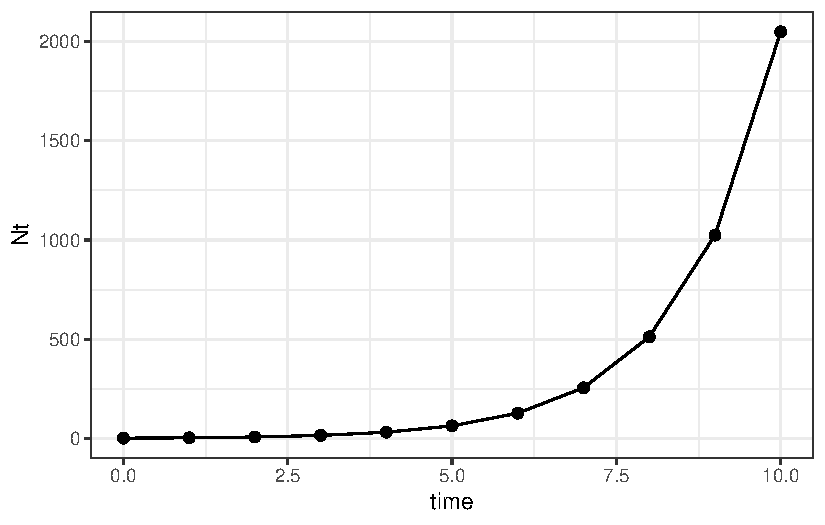
\includegraphics[keepaspectratio]{Mod_2_Activity_1_wFigs_noAI_files/figure-pdf/unnamed-chunk-2-1.pdf}}

\paragraph{Question 1: How large is the population in year
10?}\label{question-1-how-large-is-the-population-in-year-10}

The above plot shows the exponential growth for this scenario. To get
the exact population size at time 10, you will need to do a little math
using the equations above.

\paragraph{Question 2: How does starting population sizes of 2, 10, and
20 affect the final
results?}\label{question-2-how-does-starting-population-sizes-of-2-10-and-20-affect-the-final-results}

Now we will look at the effect of changing the starting population size.
Adjust the starting populations size to \(N_0\) = 10, 20, and 40 and
calculate the new answers.

\begin{Shaded}
\begin{Highlighting}[]
\DocumentationTok{\#\# lines 13{-}22 in associated R code}

\NormalTok{N0 }\OtherTok{\textless{}{-}} \FunctionTok{c}\NormalTok{(}\DecValTok{2}\NormalTok{,}\DecValTok{10}\NormalTok{,}\DecValTok{20}\NormalTok{) }
\NormalTok{lambda }\OtherTok{\textless{}{-}} \DecValTok{2}
\NormalTok{time }\OtherTok{\textless{}{-}} \DecValTok{0}\SpecialCharTok{:}\DecValTok{10}

\NormalTok{Nt.s }\OtherTok{\textless{}{-}} \FunctionTok{sapply}\NormalTok{(N0, }\ControlFlowTok{function}\NormalTok{(n) n }\SpecialCharTok{*}\NormalTok{ lambda}\SpecialCharTok{**}\NormalTok{time) }\SpecialCharTok{\%\textgreater{}\%} \FunctionTok{as.data.frame}\NormalTok{() }\SpecialCharTok{\%\textgreater{}\%} \FunctionTok{cbind}\NormalTok{(time) }\SpecialCharTok{\%\textgreater{}\%} \FunctionTok{pivot\_longer}\NormalTok{(}\AttributeTok{cols=}\DecValTok{1}\SpecialCharTok{:}\DecValTok{3}\NormalTok{, }\AttributeTok{names\_to =} \StringTok{\textquotesingle{}group\textquotesingle{}}\NormalTok{, }\AttributeTok{values\_to =} \StringTok{\textquotesingle{}N\textquotesingle{}}\NormalTok{)}

\DocumentationTok{\#\# Population sizes for the six years}
\FunctionTok{ggplot}\NormalTok{(}\AttributeTok{data=}\NormalTok{Nt.s, }\FunctionTok{aes}\NormalTok{(}\AttributeTok{x=}\NormalTok{time, }\AttributeTok{y=}\NormalTok{N, }\AttributeTok{color=}\NormalTok{group)) }\SpecialCharTok{+} 
  \FunctionTok{geom\_point}\NormalTok{() }\SpecialCharTok{+} 
  \FunctionTok{geom\_line}\NormalTok{(}\AttributeTok{linewidth =} \FloatTok{1.5}\NormalTok{) }\SpecialCharTok{+} 
  \FunctionTok{scale\_color\_viridis}\NormalTok{(}\AttributeTok{discrete =}\NormalTok{ T)}\SpecialCharTok{+}
  \FunctionTok{theme\_bw}\NormalTok{()}
\end{Highlighting}
\end{Shaded}

\pandocbounded{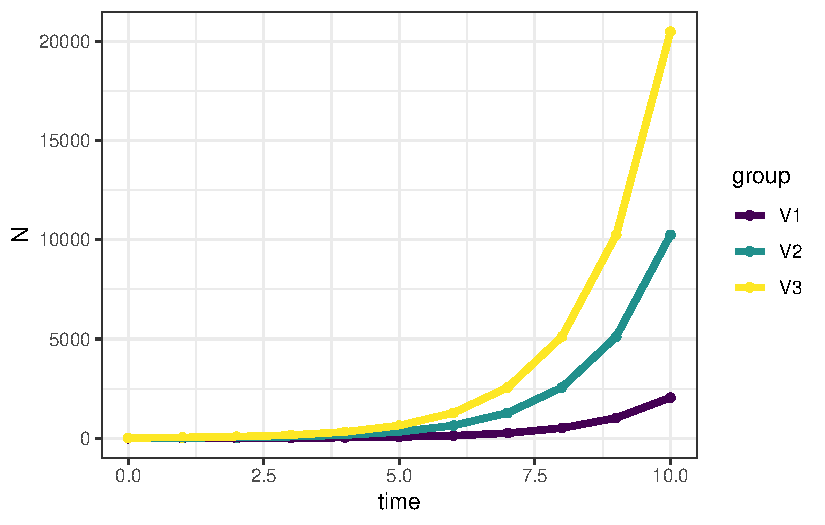
\includegraphics[keepaspectratio]{Mod_2_Activity_1_wFigs_noAI_files/figure-pdf/unnamed-chunk-3-1.pdf}}

\paragraph{Question 3: How does plotting on the log-scale change the
results? Does it affect the population sizes, or does it only change the
visualization?}\label{question-3-how-does-plotting-on-the-log-scale-change-the-results-does-it-affect-the-population-sizes-or-does-it-only-change-the-visualization}

We can also view the data on the log\_10 scale, use the plot below to
answer Question 3.

\begin{Shaded}
\begin{Highlighting}[]
\DocumentationTok{\#\# Population sizes for the six years on $log\_\{10\}$ scale}
\FunctionTok{ggplot}\NormalTok{(}\AttributeTok{data=}\NormalTok{Nt.s, }\FunctionTok{aes}\NormalTok{(}\AttributeTok{x=}\NormalTok{time, }\AttributeTok{y=}\NormalTok{N, }\AttributeTok{color=}\NormalTok{group)) }\SpecialCharTok{+} 
  \FunctionTok{geom\_point}\NormalTok{(}\AttributeTok{size=}\DecValTok{3}\NormalTok{) }\SpecialCharTok{+} 
  \FunctionTok{geom\_line}\NormalTok{(}\AttributeTok{linewidth =} \FloatTok{1.5}\NormalTok{) }\SpecialCharTok{+} 
  \FunctionTok{scale\_color\_viridis}\NormalTok{(}\AttributeTok{discrete =}\NormalTok{ T)}\SpecialCharTok{+}  
  \FunctionTok{scale\_y\_log10}\NormalTok{() }\SpecialCharTok{+} 
  \FunctionTok{theme\_bw}\NormalTok{()}
\end{Highlighting}
\end{Shaded}

\pandocbounded{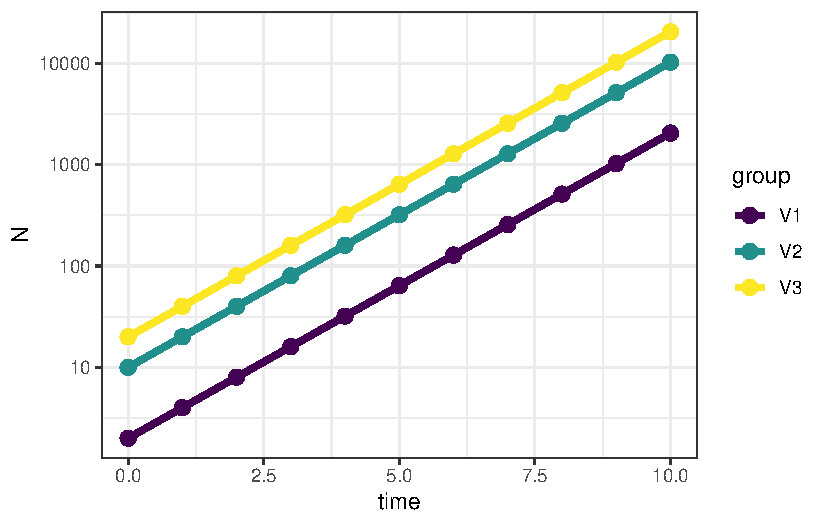
\includegraphics[keepaspectratio]{Mod_2_Activity_1_wFigs_noAI_files/figure-pdf/unnamed-chunk-4-1.pdf}}

\paragraph{Question 4: How does lambda affect population growth rates,
specifically when lamdba is above or below
1?}\label{question-4-how-does-lambda-affect-population-growth-rates-specifically-when-lamdba-is-above-or-below-1}

Below is a plot with lambda values of 0.5, 1, and 2 and the linear scale
and log-scale (second below).

\begin{Shaded}
\begin{Highlighting}[]
\DocumentationTok{\#\# lines 25{-}34 in associated R code}
\NormalTok{N0 }\OtherTok{\textless{}{-}} \DecValTok{2} 
\NormalTok{lambdas }\OtherTok{\textless{}{-}} \FunctionTok{c}\NormalTok{(}\FloatTok{0.7}\NormalTok{, }\DecValTok{1}\NormalTok{, }\FloatTok{1.5}\NormalTok{)}
\NormalTok{time }\OtherTok{\textless{}{-}} \DecValTok{0}\SpecialCharTok{:}\DecValTok{5}

\NormalTok{Nt.all }\OtherTok{\textless{}{-}} \FunctionTok{sapply}\NormalTok{(lambdas, }\ControlFlowTok{function}\NormalTok{(x) N0 }\SpecialCharTok{*}\NormalTok{ x}\SpecialCharTok{**}\NormalTok{time) }\SpecialCharTok{\%\textgreater{}\%} \FunctionTok{as.data.frame}\NormalTok{() }\SpecialCharTok{\%\textgreater{}\%} \FunctionTok{cbind}\NormalTok{(time) }\SpecialCharTok{\%\textgreater{}\%} \FunctionTok{pivot\_longer}\NormalTok{(}\AttributeTok{cols=}\DecValTok{1}\SpecialCharTok{:}\DecValTok{3}\NormalTok{, }\AttributeTok{names\_to =} \StringTok{\textquotesingle{}group\textquotesingle{}}\NormalTok{, }\AttributeTok{values\_to =} \StringTok{\textquotesingle{}N\textquotesingle{}}\NormalTok{)}

\DocumentationTok{\#\# Population sizes for the six years }
\FunctionTok{ggplot}\NormalTok{(}\AttributeTok{data=}\NormalTok{Nt.all, }\FunctionTok{aes}\NormalTok{(}\AttributeTok{x=}\NormalTok{time, }\AttributeTok{y=}\NormalTok{N, }\AttributeTok{color=}\NormalTok{group)) }\SpecialCharTok{+} 
  \FunctionTok{geom\_point}\NormalTok{(}\AttributeTok{size=}\DecValTok{3}\NormalTok{) }\SpecialCharTok{+} 
  \FunctionTok{geom\_line}\NormalTok{(}\AttributeTok{linewidth =} \FloatTok{1.5}\NormalTok{) }\SpecialCharTok{+} 
  \FunctionTok{scale\_color\_viridis}\NormalTok{(}\AttributeTok{discrete =}\NormalTok{ T)}\SpecialCharTok{+} 
  \FunctionTok{theme\_bw}\NormalTok{()}
\end{Highlighting}
\end{Shaded}

\pandocbounded{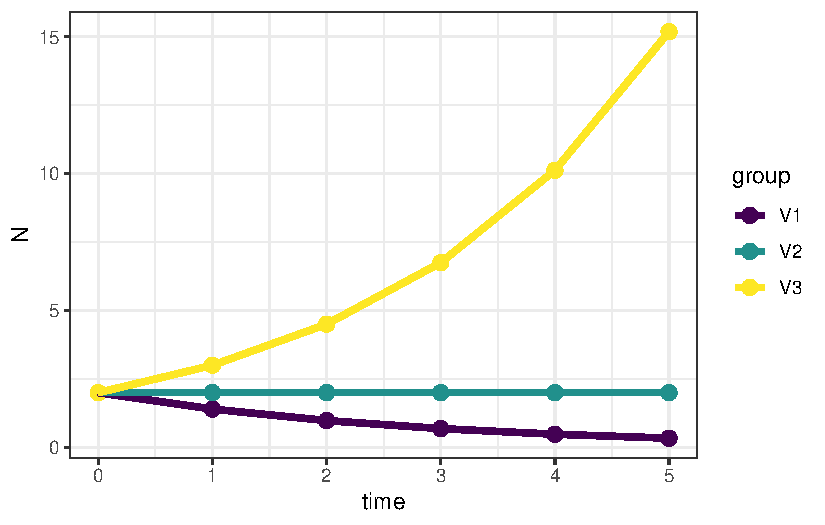
\includegraphics[keepaspectratio]{Mod_2_Activity_1_wFigs_noAI_files/figure-pdf/unnamed-chunk-5-1.pdf}}

\begin{Shaded}
\begin{Highlighting}[]
\DocumentationTok{\#\# Population sizes for the six years on $log\_\{10\}$ scale}
\FunctionTok{ggplot}\NormalTok{(}\AttributeTok{data=}\NormalTok{Nt.all, }\FunctionTok{aes}\NormalTok{(}\AttributeTok{x=}\NormalTok{time, }\AttributeTok{y=}\NormalTok{N, }\AttributeTok{color=}\NormalTok{group)) }\SpecialCharTok{+} 
  \FunctionTok{geom\_point}\NormalTok{(}\AttributeTok{size=}\DecValTok{3}\NormalTok{) }\SpecialCharTok{+} 
  \FunctionTok{geom\_line}\NormalTok{(}\AttributeTok{linewidth =} \FloatTok{1.5}\NormalTok{) }\SpecialCharTok{+} 
  \FunctionTok{scale\_color\_viridis}\NormalTok{(}\AttributeTok{discrete =}\NormalTok{ T)}\SpecialCharTok{+}  \FunctionTok{scale\_y\_log10}\NormalTok{() }\SpecialCharTok{+} 
  \FunctionTok{theme\_bw}\NormalTok{()}
\end{Highlighting}
\end{Shaded}

\pandocbounded{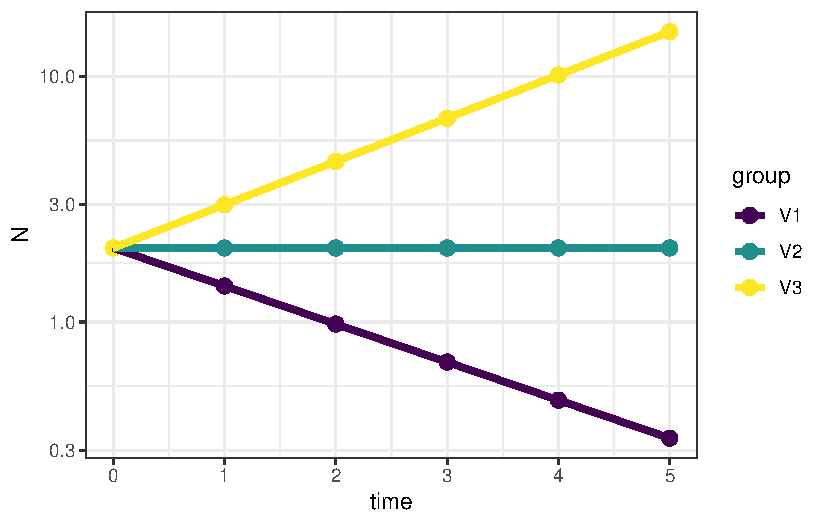
\includegraphics[keepaspectratio]{Mod_2_Activity_1_wFigs_noAI_files/figure-pdf/unnamed-chunk-5-2.pdf}}

\subsection{Part 2. Miami blue population dynamics case
study}\label{part-2.-miami-blue-population-dynamics-case-study}

\subsubsection{Part 2a. Review info about the
butterfly}\label{part-2a.-review-info-about-the-butterfly}

The Miami blue \emph{Cyclargus thomasi bethunbakeri} is an endangered
species in Florida. It was once widespread and occurred throughout much
of south Florida, but now only one small population remains in a
preserve. Read more about the biology
\href{http://entnemdept.ufl.edu/creatures/bfly/miami_blue.htm}{here}.

\begin{figure}[H]

{\centering \pandocbounded{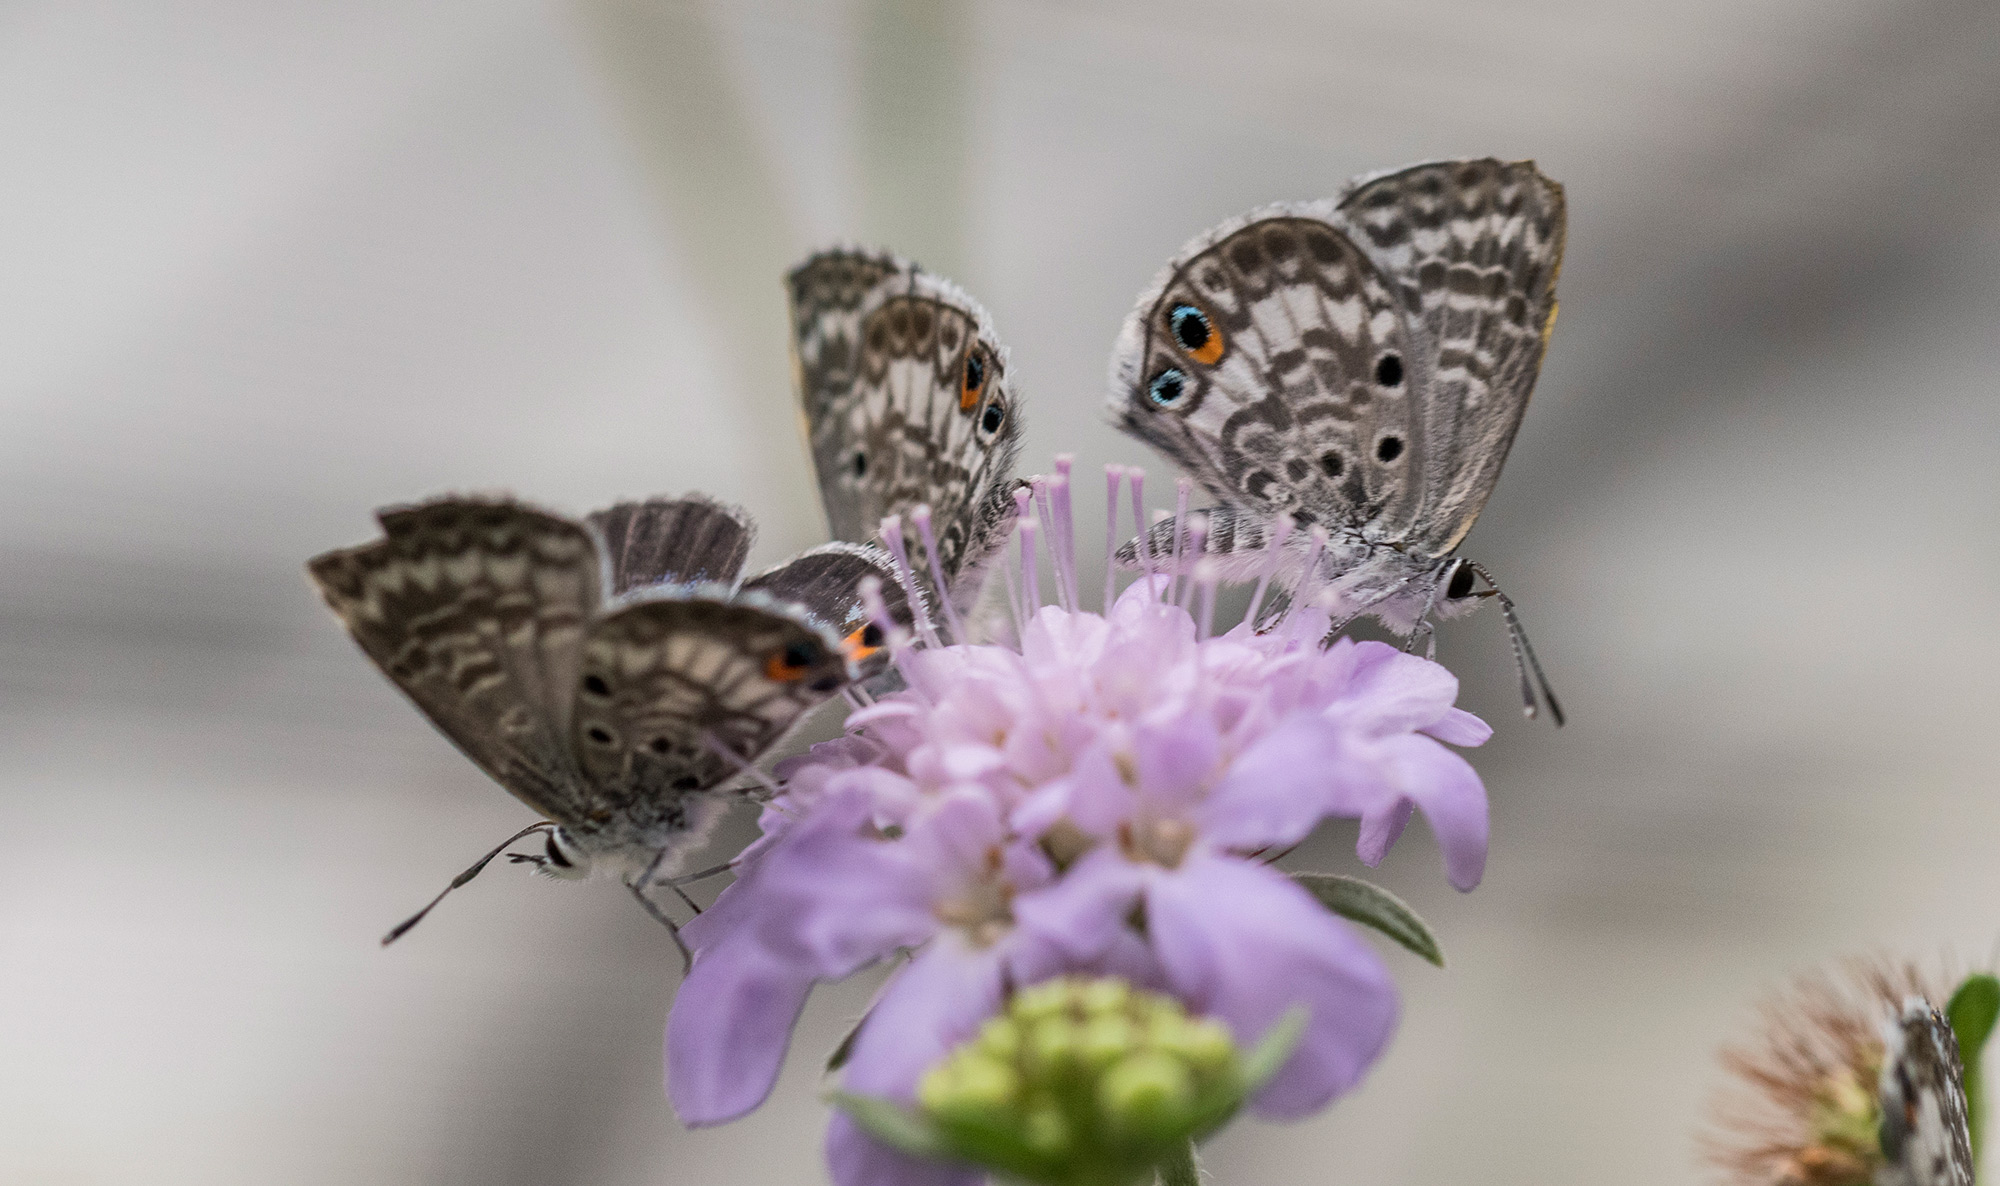
\includegraphics[keepaspectratio]{miami-blue-170302-0336.jpg}}

}

\caption{Miami blue butterflies. credit:J.Gage}

\end{figure}%

Below we will analyze data for population size counts for a the
endangered Miami blue butterfly. First,
\href{https://www.floridastateparks.org/learn/saving-miami-blue-butterfly-0}{read
more} about conservation actions being taken by the Daniels Lab here at
UF and watch the \href{https://youtu.be/d1NDRgPG4kQ}{video}.

\subsubsection{Part 2b. Examine butterfly
data}\label{part-2b.-examine-butterfly-data}

Now we will simulate 21 years of data where researchers counted the
butterflies at several sites across their range. The values are
estimated population size each year. Please note that these are
\textbf{hypothetical data} that we are simulating and do not reflect
actual abundances of the butterfly.

\begin{Shaded}
\begin{Highlighting}[]
\NormalTok{year }\OtherTok{\textless{}{-}} \DecValTok{0}\SpecialCharTok{:}\DecValTok{20}
\FunctionTok{set.seed}\NormalTok{(}\DecValTok{5}\NormalTok{)}
\NormalTok{Count }\OtherTok{\textless{}{-}} \FunctionTok{abs}\NormalTok{(}\FunctionTok{round}\NormalTok{(}\FunctionTok{rnorm}\NormalTok{(}\DecValTok{21}\NormalTok{, (}\DecValTok{100}\SpecialCharTok{*}\FloatTok{1.05}\SpecialCharTok{\^{}}\NormalTok{year), }\DecValTok{70}\NormalTok{),}\DecValTok{0}\NormalTok{))}
\NormalTok{dat }\OtherTok{\textless{}{-}} \FunctionTok{as.data.frame}\NormalTok{(}\FunctionTok{cbind}\NormalTok{(year,Count))}
\end{Highlighting}
\end{Shaded}

\paragraph{Question 5: Briefly describe your plot of 22 year population
dynamics for the Miami blue
butterfly.}\label{question-5-briefly-describe-your-plot-of-22-year-population-dynamics-for-the-miami-blue-butterfly.}

\begin{Shaded}
\begin{Highlighting}[]
\CommentTok{\# plot dynamics}
\FunctionTok{ggplot}\NormalTok{(}\AttributeTok{data=}\NormalTok{dat, }\FunctionTok{aes}\NormalTok{(}\AttributeTok{x=}\NormalTok{year, }\AttributeTok{y=}\NormalTok{Count)) }\SpecialCharTok{+} 
  \FunctionTok{geom\_point}\NormalTok{() }\SpecialCharTok{+} 
  \FunctionTok{geom\_line}\NormalTok{() }\SpecialCharTok{+} 
  \FunctionTok{theme\_bw}\NormalTok{()}
\end{Highlighting}
\end{Shaded}

\pandocbounded{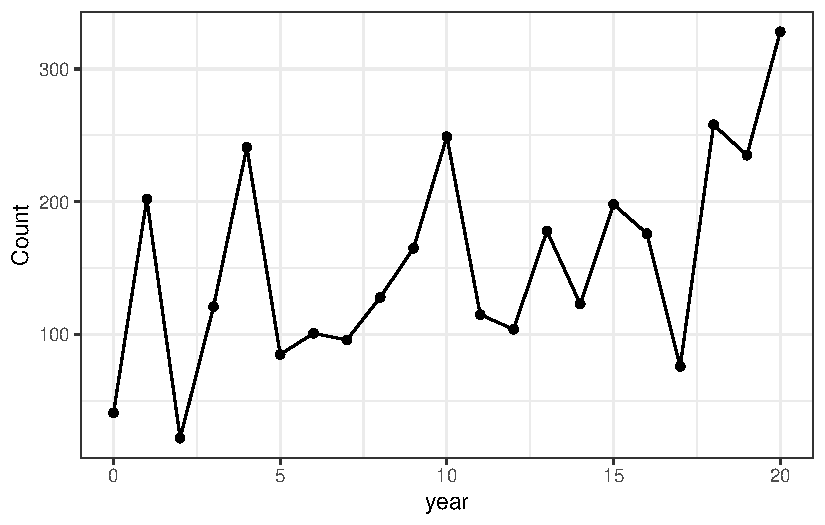
\includegraphics[keepaspectratio]{Mod_2_Activity_1_wFigs_noAI_files/figure-pdf/unnamed-chunk-7-1.pdf}}

There is quite a bit of up and down in the population numbers. We can
calculate the rate of increase (𝜆 or R) for each year-to-year
transition. Here is the plot, where `obs.R' is the increase or decrease
in each year:

\begin{Shaded}
\begin{Highlighting}[]
\NormalTok{dat}\SpecialCharTok{$}\NormalTok{obs.R }\OtherTok{\textless{}{-}} \ConstantTok{NA}

\NormalTok{dat}\SpecialCharTok{$}\NormalTok{obs.R[}\DecValTok{2}\SpecialCharTok{:}\DecValTok{21}\NormalTok{] }\OtherTok{\textless{}{-}}\NormalTok{ dat}\SpecialCharTok{$}\NormalTok{Count[}\DecValTok{2}\SpecialCharTok{:}\DecValTok{21}\NormalTok{]}\SpecialCharTok{/}\NormalTok{dat}\SpecialCharTok{$}\NormalTok{Count[}\DecValTok{1}\SpecialCharTok{:}\DecValTok{20}\NormalTok{]}
\NormalTok{obs.R }\OtherTok{\textless{}{-}}\NormalTok{ dat}\SpecialCharTok{$}\NormalTok{Count[}\DecValTok{2}\SpecialCharTok{:}\DecValTok{21}\NormalTok{]}\SpecialCharTok{/}\NormalTok{dat}\SpecialCharTok{$}\NormalTok{Count[}\DecValTok{1}\SpecialCharTok{:}\DecValTok{20}\NormalTok{]}

\FunctionTok{ggplot}\NormalTok{(}\AttributeTok{data=}\NormalTok{dat, }\FunctionTok{aes}\NormalTok{(}\AttributeTok{x=}\NormalTok{year, }\AttributeTok{y=}\NormalTok{obs.R)) }\SpecialCharTok{+} 
  \FunctionTok{geom\_point}\NormalTok{(}\AttributeTok{size=}\DecValTok{2}\NormalTok{) }\SpecialCharTok{+} 
  \FunctionTok{geom\_line}\NormalTok{() }\SpecialCharTok{+} 
  \FunctionTok{geom\_hline}\NormalTok{(}\AttributeTok{yintercept=}\DecValTok{1}\NormalTok{,}\AttributeTok{lty=}\DecValTok{2}\NormalTok{) }\SpecialCharTok{+} 
  \FunctionTok{theme\_bw}\NormalTok{()}
\end{Highlighting}
\end{Shaded}

\pandocbounded{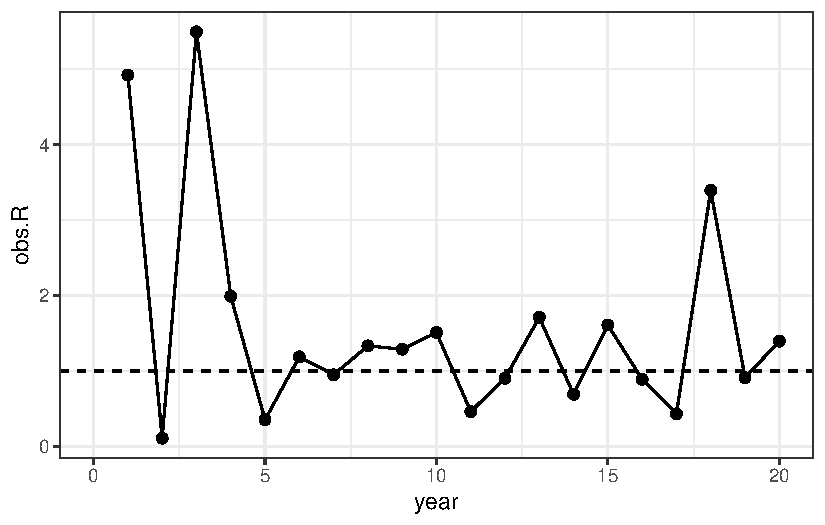
\includegraphics[keepaspectratio]{Mod_2_Activity_1_wFigs_noAI_files/figure-pdf/unnamed-chunk-8-1.pdf}}

And here is a plot showing observed R against population density of the
previous year:

\begin{Shaded}
\begin{Highlighting}[]
\FunctionTok{ggplot}\NormalTok{(}\AttributeTok{data=}\ConstantTok{NULL}\NormalTok{, }\FunctionTok{aes}\NormalTok{(}\AttributeTok{x=}\NormalTok{dat}\SpecialCharTok{$}\NormalTok{Count[}\DecValTok{1}\SpecialCharTok{:}\DecValTok{20}\NormalTok{], }\AttributeTok{y=}\NormalTok{obs.R)) }\SpecialCharTok{+} 
  \FunctionTok{geom\_point}\NormalTok{(}\AttributeTok{size=}\DecValTok{2}\NormalTok{) }\SpecialCharTok{+} \FunctionTok{geom\_abline}\NormalTok{(}\AttributeTok{intercept=}\DecValTok{1}\NormalTok{,}\AttributeTok{slope=}\DecValTok{0}\NormalTok{, }\AttributeTok{linetype=}\StringTok{"dashed"}\NormalTok{) }\SpecialCharTok{+} 
  \FunctionTok{labs}\NormalTok{(}\AttributeTok{x=}\StringTok{"Population density"}\NormalTok{,}\AttributeTok{y=}\StringTok{"observed R"}\NormalTok{)}\SpecialCharTok{+} 
  \FunctionTok{theme\_bw}\NormalTok{()}
\end{Highlighting}
\end{Shaded}

\pandocbounded{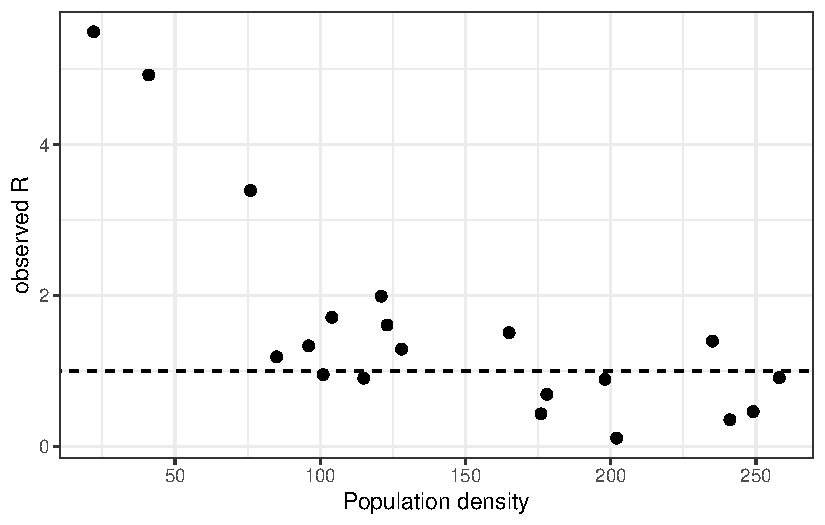
\includegraphics[keepaspectratio]{Mod_2_Activity_1_wFigs_noAI_files/figure-pdf/unnamed-chunk-9-1.pdf}}

Think about what these results imply about the population dynamics and
what may or may not regulate the populations?

\subsubsection{Part 2c. Project out population size estimates for 50
years}\label{part-2c.-project-out-population-size-estimates-for-50-years}

WWe know the population size and the rates of increase/decrease for 20
transitions that we have data for. Now we want to know what the
population size might be in 50 years. Will it substantially increase? Is
there a chance the Miami blue will go extinct? We can answer these
questions by randomly sampling from our list of 20 R's. We do this 50
times to simulate population dynamics for 50 years. What density should
we start the simulation? We could pick the average density
(\textasciitilde100) or the minimum (22). Let's be conservative and
start our simulated population at the minimum of 22 butterflies. Here is
the plot for one of these simulations:

\paragraph{Question 6: Describe your plot of the 50 year
simulation.}\label{question-6-describe-your-plot-of-the-50-year-simulation.}

\begin{Shaded}
\begin{Highlighting}[]
\DocumentationTok{\#\# lines 62{-}75 in associated R code}
\NormalTok{years }\OtherTok{\textless{}{-}} \DecValTok{0}\SpecialCharTok{:}\DecValTok{50} \CommentTok{\#setup a vector for years from 0 to 50}
\FunctionTok{set.seed}\NormalTok{(}\DecValTok{1}\NormalTok{)   }\CommentTok{\# set seed for the randomization so we can reproduce the randomized results}
\NormalTok{sim.Rs }\OtherTok{\textless{}{-}} \FunctionTok{sample}\NormalTok{(}\AttributeTok{x =}\NormalTok{ obs.R, }\AttributeTok{size =} \DecValTok{50}\NormalTok{, }\AttributeTok{replace =} \ConstantTok{TRUE}\NormalTok{) }\CommentTok{\# this line randomly samples values from \textquotesingle{}obs.R\textquotesingle{} 50 times with replacement}

\NormalTok{out50yr }\OtherTok{\textless{}{-}} \FunctionTok{numeric}\NormalTok{(}\FunctionTok{length}\NormalTok{(years))}
\NormalTok{out50yr[}\DecValTok{1}\NormalTok{] }\OtherTok{\textless{}{-}} \FunctionTok{min}\NormalTok{(dat}\SpecialCharTok{$}\NormalTok{Count) }

\ControlFlowTok{for}\NormalTok{ (t }\ControlFlowTok{in} \DecValTok{1}\SpecialCharTok{:}\DecValTok{50}\NormalTok{) out50yr[t }\SpecialCharTok{+} \DecValTok{1}\NormalTok{] }\OtherTok{\textless{}{-}}\NormalTok{ \{}
\NormalTok{  out50yr[t] }\SpecialCharTok{*}\NormalTok{ sim.Rs[t]}
\NormalTok{  \}}

\FunctionTok{ggplot}\NormalTok{(}\AttributeTok{data=}\ConstantTok{NULL}\NormalTok{, }\FunctionTok{aes}\NormalTok{(}\AttributeTok{x=}\NormalTok{years, }\AttributeTok{y=}\NormalTok{out50yr)) }\SpecialCharTok{+} 
  \FunctionTok{labs}\NormalTok{(}\AttributeTok{y=}\StringTok{"count"}\NormalTok{) }\SpecialCharTok{+} 
  \FunctionTok{geom\_point}\NormalTok{() }\SpecialCharTok{+} 
  \FunctionTok{geom\_line}\NormalTok{() }\SpecialCharTok{+} 
  \FunctionTok{theme\_bw}\NormalTok{()}
\end{Highlighting}
\end{Shaded}

\pandocbounded{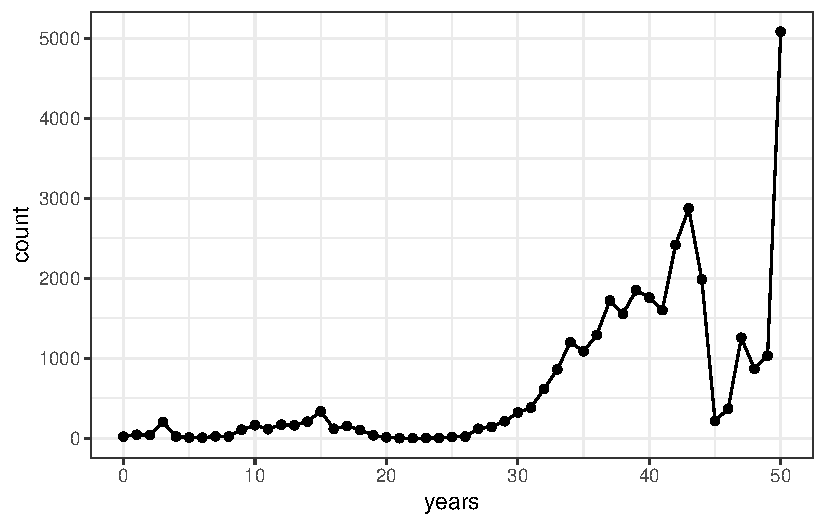
\includegraphics[keepaspectratio]{Mod_2_Activity_1_wFigs_noAI_files/figure-pdf/unnamed-chunk-10-1.pdf}}

Booming!

This is just one random simulation. We might want to do many versions of
this simulation to get an idea of how variables these results might be.
We can conduct a sensitivity analysis by running the simulations for 100
populations. From these results, calculate 1) the percent of populations
that go extinct, 2) the percent of populations that exceed 1 million
butterflies in any year, and 3) the 2.5 quantile and 4) 97.5 quantile
for the final population sizes.

Now we should see we have run 100 simulated populations, each with
dynamics for 50 years. What do we see? Are they all the same? Why or why
not? Here is a plot showing only 10 populations so its easier to see:

\begin{Shaded}
\begin{Highlighting}[]
\NormalTok{PopSim }\OtherTok{\textless{}{-}} \ControlFlowTok{function}\NormalTok{(Rs, N0, }\AttributeTok{years =} \DecValTok{50}\NormalTok{, }\AttributeTok{sims =} \DecValTok{1}\NormalTok{) \{}
\NormalTok{  sim.RM }\OtherTok{=} \FunctionTok{matrix}\NormalTok{(}\FunctionTok{sample}\NormalTok{(Rs, }\AttributeTok{size =}\NormalTok{ sims }\SpecialCharTok{*}\NormalTok{ years, }\AttributeTok{replace =} \ConstantTok{TRUE}\NormalTok{),}
                    \AttributeTok{nrow =}\NormalTok{ years, }\AttributeTok{ncol =}\NormalTok{ sims)}
\NormalTok{  output }\OtherTok{\textless{}{-}} \FunctionTok{numeric}\NormalTok{(years }\SpecialCharTok{+} \DecValTok{1}\NormalTok{)}
\NormalTok{  output[}\DecValTok{1}\NormalTok{] }\OtherTok{\textless{}{-}}\NormalTok{ N0}
\NormalTok{  outmat }\OtherTok{\textless{}{-}} \FunctionTok{sapply}\NormalTok{(}\DecValTok{1}\SpecialCharTok{:}\NormalTok{sims, }\ControlFlowTok{function}\NormalTok{(i) \{}
    \ControlFlowTok{for}\NormalTok{ (t }\ControlFlowTok{in} \DecValTok{1}\SpecialCharTok{:}\NormalTok{years) output[t }\SpecialCharTok{+} \DecValTok{1}\NormalTok{] }\OtherTok{\textless{}{-}} \FunctionTok{round}\NormalTok{(output[t] }\SpecialCharTok{*}\NormalTok{ sim.RM[t, i], }\DecValTok{0}\NormalTok{)}
\NormalTok{    output}
\NormalTok{    \})}
  \FunctionTok{return}\NormalTok{(}\FunctionTok{as.data.frame}\NormalTok{(outmat))}
\NormalTok{\}}
\end{Highlighting}
\end{Shaded}

Some of the populations are so big that it's hard to see the patterns
for some of the populations. Probably you coding assistant will plot the
data on both the linear and log scale so you can visualize them better.
If not, you may need to ask for the plots on the log scale.

\begin{Shaded}
\begin{Highlighting}[]
\DocumentationTok{\#\# lines 92{-}100 in associated R code}
\NormalTok{sim10 }\OtherTok{\textless{}{-}} \FunctionTok{as\_tibble}\NormalTok{(}\FunctionTok{PopSim}\NormalTok{(}\AttributeTok{Rs =}\NormalTok{ obs.R, }\AttributeTok{N0 =} \DecValTok{43}\NormalTok{, }\AttributeTok{sims =} \DecValTok{100}\NormalTok{)) }\SpecialCharTok{\%\textgreater{}\%}
  \FunctionTok{mutate}\NormalTok{(}\AttributeTok{year =} \DecValTok{0}\SpecialCharTok{:}\DecValTok{50}\NormalTok{) }\SpecialCharTok{\%\textgreater{}\%}
  \FunctionTok{pivot\_longer}\NormalTok{(}\SpecialCharTok{{-}}\NormalTok{year, }\AttributeTok{names\_to =} \StringTok{"sim"}\NormalTok{, }\AttributeTok{values\_to =} \StringTok{"count"}\NormalTok{) }\SpecialCharTok{\%\textgreater{}\%}
  \FunctionTok{as.data.frame}\NormalTok{() }\SpecialCharTok{\%\textgreater{}\%}
\NormalTok{  \{}\FunctionTok{data.frame}\NormalTok{(., }\AttributeTok{row.names =} \ConstantTok{NULL}\NormalTok{)\}}

\CommentTok{\# plot the 10 simulated populations}
\FunctionTok{ggplot}\NormalTok{(sim10, }\FunctionTok{aes}\NormalTok{(}\AttributeTok{x=}\NormalTok{year,}\AttributeTok{y=}\NormalTok{count,}\AttributeTok{color=}\NormalTok{sim))}\SpecialCharTok{+}
  \FunctionTok{geom\_line}\NormalTok{(}\AttributeTok{linewidth =} \DecValTok{1}\NormalTok{) }\SpecialCharTok{+} 
  \FunctionTok{scale\_color\_viridis}\NormalTok{(}\AttributeTok{discrete =}\NormalTok{ T)}\SpecialCharTok{+}  \FunctionTok{theme\_bw}\NormalTok{()}\SpecialCharTok{+} 
  \FunctionTok{theme}\NormalTok{(}\AttributeTok{legend.position =} \StringTok{"none"}\NormalTok{)}
\end{Highlighting}
\end{Shaded}

\pandocbounded{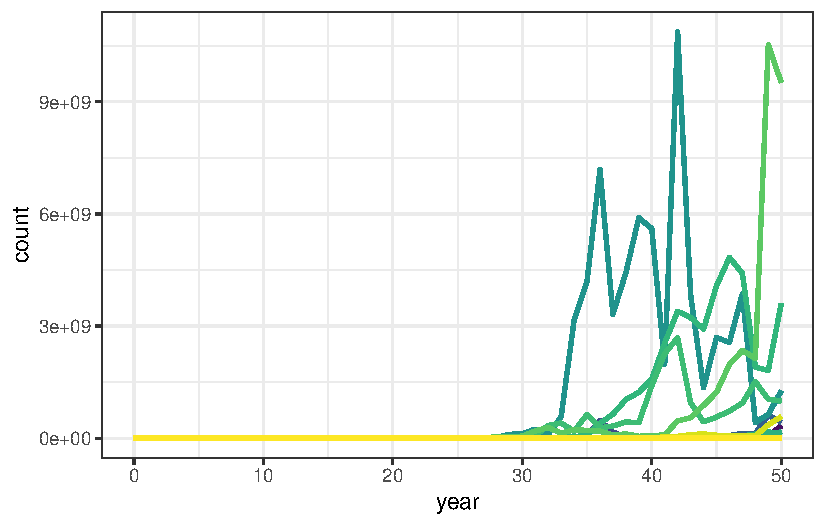
\includegraphics[keepaspectratio]{Mod_2_Activity_1_wFigs_noAI_files/figure-pdf/unnamed-chunk-12-1.pdf}}

\begin{Shaded}
\begin{Highlighting}[]
\FunctionTok{ggplot}\NormalTok{(sim10, }\FunctionTok{aes}\NormalTok{(}\AttributeTok{x=}\NormalTok{year,}\AttributeTok{y=}\FunctionTok{log}\NormalTok{(count}\SpecialCharTok{+}\DecValTok{1}\NormalTok{),}\AttributeTok{color=}\NormalTok{sim))}\SpecialCharTok{+}
  \FunctionTok{geom\_line}\NormalTok{(}\AttributeTok{linewidth =} \FloatTok{0.75}\NormalTok{, }\AttributeTok{alpha=}\FloatTok{0.75}\NormalTok{) }\SpecialCharTok{+} 
  \FunctionTok{scale\_color\_viridis}\NormalTok{(}\AttributeTok{discrete =}\NormalTok{ T)}\SpecialCharTok{+}  
  \FunctionTok{theme\_bw}\NormalTok{() }\SpecialCharTok{+} 
  \FunctionTok{theme}\NormalTok{(}\AttributeTok{legend.position =} \StringTok{"none"}\NormalTok{)}
\end{Highlighting}
\end{Shaded}

\pandocbounded{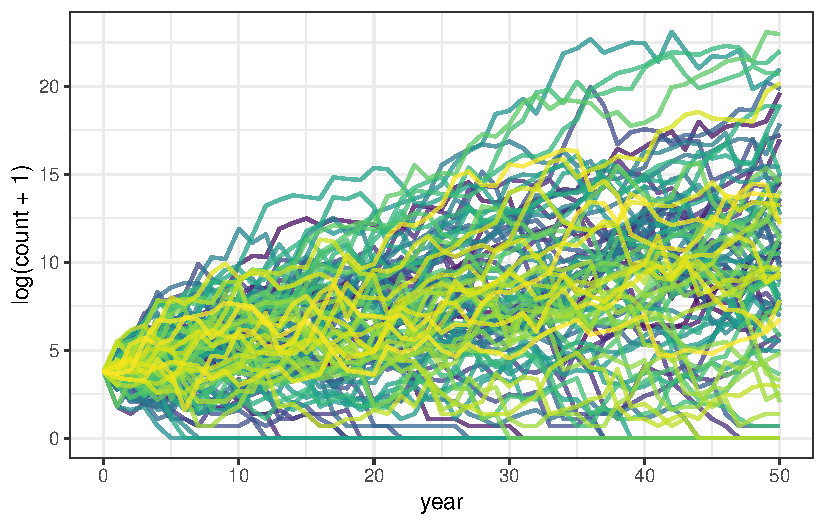
\includegraphics[keepaspectratio]{Mod_2_Activity_1_wFigs_noAI_files/figure-pdf/unnamed-chunk-13-1.pdf}}

\begin{Shaded}
\begin{Highlighting}[]
\NormalTok{year50\_data }\OtherTok{\textless{}{-}}\NormalTok{ sim10[sim10}\SpecialCharTok{$}\NormalTok{year }\SpecialCharTok{==} \DecValTok{50}\NormalTok{, ]}

\FunctionTok{data.frame}\NormalTok{(}
  \AttributeTok{n\_extinct =} \FunctionTok{sum}\NormalTok{(year50\_data}\SpecialCharTok{$}\NormalTok{count }\SpecialCharTok{==} \DecValTok{0}\NormalTok{),}
  \AttributeTok{n\_greater\_1mil =} \FunctionTok{sum}\NormalTok{(year50\_data}\SpecialCharTok{$}\NormalTok{count }\SpecialCharTok{\textgreater{}} \DecValTok{1000000}\NormalTok{),}
  \AttributeTok{q02.5 =} \FunctionTok{quantile}\NormalTok{(year50\_data}\SpecialCharTok{$}\NormalTok{count, }\AttributeTok{probs =} \FloatTok{0.025}\NormalTok{),}
  \AttributeTok{q97.5 =} \FunctionTok{quantile}\NormalTok{(year50\_data}\SpecialCharTok{$}\NormalTok{count, }\AttributeTok{probs =} \FloatTok{0.975}\NormalTok{)}
\NormalTok{)}
\end{Highlighting}
\end{Shaded}

\begin{verbatim}
     n_extinct n_greater_1mil q02.5      q97.5
2.5%        18             21     0 1135061538
\end{verbatim}

\paragraph{Question 7: From these results, what are the values for the
following
calculations:}\label{question-7-from-these-results-what-are-the-values-for-the-following-calculations}

\begin{enumerate}
\def\labelenumi{\arabic{enumi})}
\tightlist
\item
  the percent of populations that go extinct?
\item
  the percent of populations that exceed 1 million butterflies in any
  year?
\item
  the 2.5 and 97.5 quantiles for the final population sizes?
\end{enumerate}

\paragraph{Question 8. Write a brief summary of your results (100-150
words) that you might communicate to a land manager about the Miami Blue
population dynamics and the potential for extinction. Specifically
mention whether you think this is a realistic
scenario.}\label{question-8.-write-a-brief-summary-of-your-results-100-150-words-that-you-might-communicate-to-a-land-manager-about-the-miami-blue-population-dynamics-and-the-potential-for-extinction.-specifically-mention-whether-you-think-this-is-a-realistic-scenario.}

\paragraph{Question 9-10. These question is not relevant for this
version, please just enter ``NA'' or
skip}\label{question-9-10.-these-question-is-not-relevant-for-this-version-please-just-enter-na-or-skip}




\end{document}
